\documentclass[11pt]{amsart}

\usepackage[T1]{fontenc}
\usepackage{lmodern}
\usepackage{amssymb,amsmath}
\usepackage{graphicx}
\usepackage[dvipsnames]{xcolor}
\usepackage[margin=1.15in]{geometry}
\usepackage[colorlinks=true,linkcolor=blue!50!black,citecolor=blue!50!black,urlcolor=blue!50!black]{hyperref}

\newtheorem{theorem}{Theorem}[section]
\newtheorem{proposition}[theorem]{Proposition}
\newtheorem{lemma}[theorem]{Lemma}
\newtheorem{corollary}[theorem]{Corollary}
\theoremstyle{definition}
\newtheorem{definition}[theorem]{Definition}
\newtheorem{innerconj}{Conjecture}
\newenvironment{conjecture}[1]{\renewcommand{\theinnerconj}{#1}\innerconj}{\endinnerconj}
\theoremstyle{remark}
\newtheorem{remark}[theorem]{Remark}

\numberwithin{equation}{section}

\newcommand{\tb}{\bar\tau}
\hypersetup{pdftitle={All tau\_k-maximal graphs have the same size},pdfauthor={Deep Bhattacharjee}}
\providecommand{\doi}[1]{\url{https://doi.org/#1}}

\begin{document}

\title[All \texorpdfstring{$\tau_{\lowercase{k}}$}{tau\_k}-maximal graphs have the same size]{All \texorpdfstring{$\tau_{\lowercase{k}}$}{tau\_k}-maximal graphs have the same size}

\author{Deep Bhattacharjee}
\address{Formerly, Electro-Gravitational Space Propulsion Laboratory (EGSPL),\newline Bhubaneswar, Odisha 751030, India}
\email{d.bhattacharjee@erl-forschung.de}
\email{itsdeep@live.com}
\urladdr{https://orcid.org/0000-0003-0466-750X}
\thanks{Corresponding author: \href{mailto:d.bhattacharjee@erl-forschung.de}{d.bhattacharjee@erl-forschung.de}; ORCID \href{https://orcid.org/0000-0003-0466-750X}{\mbox{0000-0003-0466-750X}}}

\subjclass[2020]{Primary 05C05; Secondary 05C35, 05B35}
\keywords{edge-disjoint spanning trees, saturated graphs, sparse graphs, count matroid}

\begin{abstract}
A graph is $\tau_k$-maximal if none of its subgraphs has $k+1$ edge-disjoint spanning trees, but adding any missing edge creates such a subgraph. Wang and Tian conjectured that every $\tau_k$-maximal graph on $n\ge 2k+2$ vertices has exactly $(k+1)(n-1)-1$ edges. We prove this conjecture.
\end{abstract}

\maketitle

\section{Introduction}

All graphs in this note are finite and simple. For a graph $H$ with at least two vertices, $\tau(H)$ denotes the largest number of edge-disjoint spanning trees of $H$, and for a graph $G$ we put
\[
\tb(G)=\max\{\tau(H): H\subseteq G,\ |V(H)|\ge 2\}.
\]
Adding an edge raises $\tb$ by at most one. Following Wang and Tian~\cite{WT}, a graph $G$ is \emph{$\tau_k$-maximal} if $\tb(G)\le k$ while $\tb(G+e)\ge k+1$ for every edge $e$ of the complement of $G$. Since $\tau(K_n)=\lfloor n/2\rfloor$, the complete graph $K_n$ is the only $\tau_k$-maximal graph on $n\le 2k+1$ vertices, so the interesting range is $n\ge 2k+2$. There Wang and Tian proved that a $\tau_k$-maximal graph has at most $(k+1)(n-1)-1$ edges, built a family of $\tau_k$-maximal graphs with exactly that many edges, and proved that every $\tau_1$-maximal graph on $n$ vertices has $2n-3$ edges. They proposed the following statement~\cite[Conjecture~1]{WT}.

\begin{conjecture}{1}\label{conj}
Let $k\ge1$ and $n\ge 2k+2$. Every $\tau_k$-maximal graph of order $n$ has exactly $(k+1)(n-1)-1$ edges.
\end{conjecture}

We prove it, together with a description of the $\tau_k$-maximal graphs by counting alone. For $X\subseteq V(G)$ let $e_G(X)$ be the number of edges of $G$ with both ends in $X$.

\begin{theorem}\label{thm:main}
Let $k\ge1$ and $n\ge2k+2$, and let $G$ be a graph with $n$ vertices. The following are equivalent.
\begin{enumerate}
\item[(a)] $G$ is $\tau_k$-maximal.
\item[(b)] $|E(G)|=(k+1)(n-1)-1$, and $e_G(X)\le (k+1)(|X|-1)-1$ for every $X\subseteq V(G)$ with $|X|\ge2$.
\end{enumerate}
In particular, Conjecture~\ref{conj} is true.
\end{theorem}

The proof has three steps. Section~\ref{sec:sparse} turns the condition $\tb(G)\le k$ into a counting condition, using the theorem of Nash-Williams and Tutte. Section~\ref{sec:tight} shows, by an exchange argument with tight sets, that all maximal edge sets satisfying the counting condition have the same size; in the language of matroids they are the bases of a count matroid. Section~\ref{sec:rank} computes the common size with one explicit example.

\section{The counting condition}\label{sec:sparse}

Throughout, $a=k+1\ge 2$. Call a graph $G$ \emph{$a$-sparse} if
\begin{equation}\label{eq:sparse}
e_G(X)\le a(|X|-1)-1\qquad\text{for every }X\subseteq V(G)\text{ with }|X|\ge2 .
\end{equation}
We use the theorem of Nash-Williams~\cite{NW} and Tutte~\cite{Tutte}: a graph $H$ has $a$ edge-disjoint spanning trees if and only if, for every partition $\mathcal P$ of $V(H)$ into $t$ parts, at least $a(t-1)$ edges of $H$ join different parts.

\begin{lemma}\label{lem:sparse}
For every graph $G$, $\tb(G)\le k$ if and only if $G$ is $(k+1)$-sparse.
\end{lemma}

\begin{proof}
If a subgraph $H$ of $G$ on a vertex set $X$ with $|X|\ge2$ has $a$ edge-disjoint spanning trees, then $e_G(X)\ge|E(H)|\ge a(|X|-1)$, and \eqref{eq:sparse} fails for $X$.

Conversely, suppose \eqref{eq:sparse} fails, and choose a set $X$ with $|X|\ge2$ and $e_G(X)\ge a(|X|-1)$ with $|X|$ as small as possible. Let $\mathcal P=\{P_1,\dots,P_t\}$ be a partition of $X$ with $t\ge2$. A part with at least two vertices is a smaller set than $X$, so by the choice of $X$ it spans at most $a(|P_i|-1)-1<a(|P_i|-1)$ edges; a part with one vertex spans $0=a(|P_i|-1)$ edges. Hence the number of edges of $G[X]$ joining different parts is at least
\[
e_G(X)-\sum_{i=1}^t a(|P_i|-1)\ \ge\ a(|X|-1)-a(|X|-t)=a(t-1).
\]
By the theorem of Nash-Williams and Tutte, $G[X]$ has $a$ edge-disjoint spanning trees, so $\tb(G)\ge a=k+1$.
\end{proof}

By Lemma~\ref{lem:sparse}, a graph $G$ on the vertex set $V$ of $K_n$ is $\tau_k$-maximal exactly when $E(G)$ is $(k+1)$-sparse and $E(G)\cup\{e\}$ is not, for every edge $e$ of $K_n$ outside $E(G)$. In other words, $E(G)$ is a maximal sparse subset of $E(K_n)$; here and below we call a set $F$ of edges sparse when the graph $(V,F)$ is $a$-sparse.

\section{Tight sets}\label{sec:tight}

Fix a sparse set $I$ of edges of $K_n$, and write $e(X)=e_I(X)$. A set $X\subseteq V$ with $|X|\ge2$ is \emph{tight} if $e(X)=a(|X|-1)-1$, that is, if \eqref{eq:sparse} holds for $X$ with equality.

\begin{lemma}\label{lem:tight}
\begin{enumerate}
\item[(i)] $e(X\cup Y)+e(X\cap Y)\ge e(X)+e(Y)$ for all $X,Y\subseteq V$.
\item[(ii)] If $X$ and $Y$ are tight and $|X\cap Y|\ge2$, then $X\cup Y$ is tight.
\item[(iii)] If $uv$ is an edge of $K_n$ outside $I$ and $I\cup\{uv\}$ is not sparse, then some tight set contains both $u$ and $v$.
\end{enumerate}
\end{lemma}

\begin{proof}
(i) An edge counted in $e(X)$ or in $e(Y)$ lies inside $X\cup Y$, and an edge counted in both lies inside $X\cap Y$.

(ii) Since $|X\cap Y|\ge2$, the set $X\cap Y$ satisfies \eqref{eq:sparse}, and by (i)
\[
e(X\cup Y)\ \ge\ \bigl(a(|X|-1)-1\bigr)+\bigl(a(|Y|-1)-1\bigr)-\bigl(a(|X\cap Y|-1)-1\bigr)=a(|X\cup Y|-1)-1 .
\]
The reverse inequality is \eqref{eq:sparse} for $X\cup Y$.

(iii) Some $X$ with $|X|\ge2$ has more than $a(|X|-1)-1$ edges of $I\cup\{uv\}$ inside it, and at most $a(|X|-1)-1$ edges of $I$. So $uv$ lies inside $X$, and $X$ is tight.
\end{proof}

\begin{lemma}\label{lem:exchange}
Let $I$ be a maximal sparse subset of $E(K_n)$ and let $J$ be any sparse subset. Then $|J|\le|I|$.
\end{lemma}

\begin{proof}
Tight sets refer to $I$. Let $M_1,\dots,M_p$ be the tight sets that are maximal under inclusion; every tight set lies inside one of them. If $|M_i\cap M_j|\ge2$, then $M_i\cup M_j$ is tight and contains both, so $M_i=M_i\cup M_j=M_j$. Hence two different sets $M_i$ share at most one vertex, and every edge of $K_n$ lies inside at most one of them. Moreover, if $uv\notin I$, then $I\cup\{uv\}$ is not sparse because $I$ is maximal, so by Lemma~\ref{lem:tight}(iii) the pair $uv$ lies inside some $M_i$.

Let $R$ be the set of edges of $K_n$ lying inside no $M_i$; by what we just proved, $R\subseteq I$. Counting the edges of $J$ according to the set $M_i$ they lie in,
\[
|J|=\sum_{i=1}^p e_J(M_i)+|J\cap R|\ \le\ \sum_{i=1}^p\bigl(a(|M_i|-1)-1\bigr)+|R|=\sum_{i=1}^p e_I(M_i)+|I\cap R|=|I| .
\]
Here $e_J(M_i)\le a(|M_i|-1)-1$ because $J$ is sparse, and $a(|M_i|-1)-1=e_I(M_i)$ because $M_i$ is tight.
\end{proof}

Applying Lemma~\ref{lem:exchange} in both directions gives the following.

\begin{corollary}\label{cor:same}
All maximal sparse subsets of $E(K_n)$ have the same size $r$, the largest size of a sparse subset. A graph on $n$ vertices is $\tau_k$-maximal if and only if it is $(k+1)$-sparse and has exactly $r$ edges.
\end{corollary}

\begin{remark}
In the language of matroids, Lemma~\ref{lem:exchange} says that the sparse sets are the independent sets of a matroid on $E(K_n)$. This is a special case of a theorem of Edmonds~\cite{Edmonds} on matroids defined by submodular functions, and such count matroids are well known in rigidity theory~\cite{LS,Whiteley}. The direct argument above keeps the note self-contained.
\end{remark}

\section{The rank}\label{sec:rank}

Taking $X=V$ in \eqref{eq:sparse} shows $r\le a(n-1)-1$. For the reverse inequality we need one sparse graph with $a(n-1)-1$ edges; Wang and Tian give a family of them~\cite{WT}, and the following one is quick to check.

\begin{lemma}\label{lem:example}
Let $n\ge 2a$. Split the vertex set into $A$ with $|A|=a$ and $B$ with $|B|=n-a\ge a$, fix $W\subseteq B$ with $|W|=a$, and fix two vertices $w,w'$ of $W$. Let $G_0$ have as edges all pairs inside $A$, all pairs between $A$ and $B$, and all pairs inside $W$ except $ww'$ (Figure~\ref{fig:g0}). Then $G_0$ is $a$-sparse and has $a(n-1)-1$ edges.
\end{lemma}

\begin{figure}[ht]
\centering
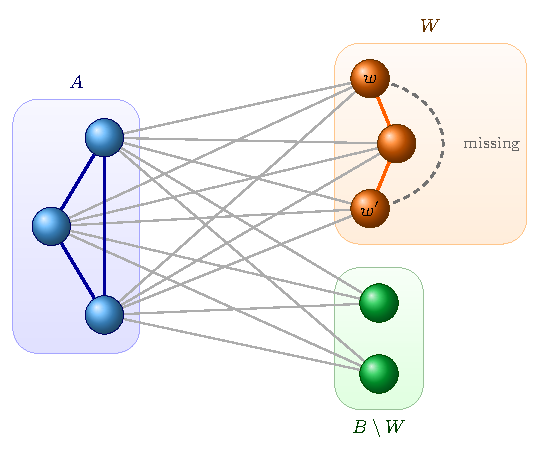
\includegraphics[width=0.62\textwidth]{figures/g0}
\caption{The graph $G_0$ for $a=3$ and $n=8$. On $A\cup W$ it is the complete graph $K_6$ without the edge $ww'$, and each vertex of $B\setminus W$ is joined to the three vertices of $A$. It has $20=3\cdot7-1$ edges.}
\label{fig:g0}
\end{figure}

\begin{proof}
The number of edges is $\binom a2+a(n-a)+\binom a2-1=a(n-1)-1$.

Put $C=A\cup W$. On $C$ the graph $G_0$ is the complete graph on $2a$ vertices without the edge $ww'$, and each vertex outside $C$ is adjacent exactly to the vertices of $A$. We first check \eqref{eq:sparse} for sets $Y\subseteq C$ with $y=|Y|\ge2$. If $y=2a$, then $Y=C$ and $e_{G_0}(Y)=\binom{2a}2-1=a(2a-1)-1$, which is \eqref{eq:sparse} with equality. If $y\le 2a-1$, then $(y-1)(2a-y)\ge2$: for $y=2$ the product is $2a-2\ge2$, and for $y\ge3$ the first factor is at least $2$ and the second at least $1$. This rearranges to $y(y-1)\le 2a(y-1)-2$, so
\[
e_{G_0}(Y)\le\binom y2\le a(y-1)-1 .
\]

Now let $X\subseteq V$ with $|X|\ge2$, and put $Y=X\cap C$ and $Z=X\setminus C$. There are no edges inside $Z$, and a vertex of $Z$ has at most $|X\cap A|\le\min(a,|Y|)$ neighbours in $X$. Hence
\[
e_{G_0}(X)\le e_{G_0}(Y)+|Z|\min(a,|Y|).
\]
If $|Y|\ge2$, this is at most $a(|Y|-1)-1+a|Z|=a(|X|-1)-1$. If $|Y|=1$, it is at most $|Z|\le a|Z|-1=a(|X|-1)-1$, as $|Z|\ge1$ and $a\ge2$. If $Y=\emptyset$, it is $0\le a(|X|-1)-1$.
\end{proof}

\begin{proof}[Proof of Theorem~\ref{thm:main}]
By Lemma~\ref{lem:example} and the upper bound above, $r=a(n-1)-1=(k+1)(n-1)-1$ when $n\ge 2k+2$. Corollary~\ref{cor:same} now says that $G$ is $\tau_k$-maximal exactly when it is $(k+1)$-sparse and has $(k+1)(n-1)-1$ edges, which is condition~(b).
\end{proof}

\begin{remark}
Lemma~\ref{lem:sparse} holds for every $n$, and for $n\le 2k+1$ the whole edge set of $K_n$ is $(k+1)$-sparse, since a set $X$ with $2\le|X|\le 2k+1$ spans $\binom{|X|}2\le(k+1)(|X|-1)-1$ edges. So in that range the rank is $\binom n2$ and $K_n$ is the only $\tau_k$-maximal graph, in line with the observation of Wang and Tian. The proof above also gives back their upper bound and their result for $k=1$.
\end{remark}

\begin{remark}
For $k=1$, condition (b) says $|E(G)|=2n-3$ and $e_G(X)\le 2|X|-3$ whenever $|X|\ge2$. These are the Laman graphs, the generically minimally rigid graphs in the plane~\cite{Laman}. So the $\tau_1$-maximal graphs are exactly the Laman graphs, and in general the $\tau_k$-maximal graphs are the bases of the $(k+1,k+2)$ count matroid.
\end{remark}

\begin{remark}
Theorem~\ref{thm:main} also says that a $\tau_k$-maximal graph can be grown greedily: starting from any $(k+1)$-sparse graph on $n\ge 2k+2$ vertices and adding edges one at a time as long as the graph stays sparse always ends with $(k+1)(n-1)-1$ edges. Whether a given set of edges is sparse can be decided in polynomial time, for instance with the pebble game of Lee and Streinu~\cite{LS}.
\end{remark}

\subsection*{Use of generative AI} The author used Claude (Anthropic) for literature search, computation and drafting; the author checked the mathematics and takes full responsibility for the content.

\begin{thebibliography}{9}

\bibitem{Edmonds}
J.~Edmonds, \emph{Submodular functions, matroids, and certain polyhedra}, in: Combinatorial Structures and their Applications (Calgary, 1969), Gordon and Breach, New York, 1970, pp.~69--87. Reprinted in: Combinatorial Optimization---Eureka, You Shrink!, Lecture Notes in Comput. Sci. \textbf{2570}, Springer, Berlin, 2003, pp.~11--26. \doi{10.1007/3-540-36478-1_2}

\bibitem{Laman}
G.~Laman, \emph{On graphs and rigidity of plane skeletal structures}, J. Engrg. Math. \textbf{4} (1970), 331--340. \doi{10.1007/BF01534980}

\bibitem{LS}
A.~Lee and I.~Streinu, \emph{Pebble game algorithms and sparse graphs}, Discrete Math. \textbf{308} (2008), 1425--1437. \doi{10.1016/j.disc.2007.07.104}

\bibitem{NW}
C.~St.~J.~A. Nash-Williams, \emph{Edge-disjoint spanning trees of finite graphs}, J. London Math. Soc. \textbf{36} (1961), 445--450. \doi{10.1112/jlms/s1-36.1.445}

\bibitem{Tutte}
W.~T. Tutte, \emph{On the problem of decomposing a graph into $n$ connected factors}, J. London Math. Soc. \textbf{36} (1961), 221--230. \doi{10.1112/jlms/s1-36.1.221}

\bibitem{WT}
Q.~Wang and Y.~Tian, \emph{Extremal graphs with no subgraph admitting $k+1$ edge-disjoint spanning trees}, preprint, 2026. \href{https://arxiv.org/abs/2606.28198}{arXiv:2606.28198}

\bibitem{Whiteley}
W.~Whiteley, \emph{Some matroids from discrete applied geometry}, in: Matroid Theory (Seattle, 1995), Contemp. Math. \textbf{197}, Amer. Math. Soc., Providence, RI, 1996, pp.~171--311. \doi{10.1090/conm/197/02540}

\end{thebibliography}

\end{document}
